\subsection{Elderly Persona}
\label{sub:elderly_persona}

\marginpar{%
	\smallskip
	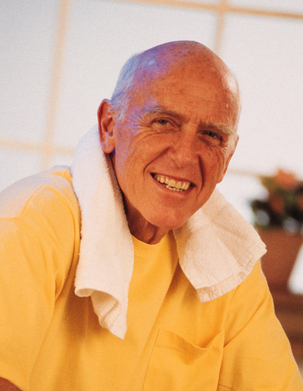
\includegraphics[width=\marginparwidth]{img/personas/elderly.jpg}
	\medskip
	\begin{description}[leftmargin=3cm]
		\item[Name] Howard Evans
		\item[Occupation] Retired
		\item[Age] 65
	\end{description}

	\subsection*{Main Goals}
	\begin{itemize}[leftmargin=1em]
		\item Increase his overall physical activity.
		\item Maintain his independence from his wife.
		\item Limit his time using computers.
		\item Pay for the activity at the venue.
	\end{itemize}
}

\subsubsection*{Description}
\label{ssub:eldery_description}

Howard lives on the outskirts of York with his wife. Howard's wife works most
days of the week as a supermarket shop assistant and their youngest son has now
left home for university in London, leaving Howard with a lot of spare time on
his hands. To help stay connected with his dad, Howard’s son has bought him a
smartphone in spite of Howard’s inexperience and frustration with technology.
For this reason he also prefers not to put any sensitive information in his
phone, like credit card information.

Though Howard was very active in his working years, he has come to enjoy a more
sedate life since retiring last year from his job as a construction manager.
Recently diagnosed with osteoarthritis, Howard has been advised to exercise
more regularly to help strengthen his muscles and joints. Howard has always
been competitive, and would happily try his hand at any sport he could find.
However, joint pain in his knees often restricts him from some high impact
activities.

No longer able to drive, Howard relies on walking and public transport to get
around during the week when his wife is not at home to drive him.

% subsubsection description (end)

\subsubsection*{Scenarios}
\label{ssub:eldery_scenarios}

\begin{itemize}
	\item Howard's doctor has just told him he needs to start doing more
		activity. Howard has a lot of free time, but he doesn’t know what
		sports he wants to play and doesn’t know what facilities there are in
		York so he searches on his phone to see what his options are.

	\item Howard has gathered a group of 4 old friends to play sport with him
		this Friday when they are all free. They're happy to play anything
		involving a racquet. If it goes well, he wants to make it a regularly
		weekly activity.

	\item Howard has been having a lot of knee pain over the last few days so
		his doctor has suggested he try swimming. He doesn’t think he can
		travel too far from his house and is worried he would need disabled
		access at the pool and doesn’t want to feel rushed at the pool by
		younger and faster swimmers.
\end{itemize}

% subsubsection scenarios (end)

\subsubsection*{Pain Points}
\label{ssub:eldery_pain_points}

\begin{itemize}
	\item joint pain in his hands often causes difficulty and discomfort when
		using his mobile phone.
	\item has very little patience with technology.
	\item would often prefer to play close to public transport facilities.
	\item joint pain in his knees often makes walking up stairs very
		uncomfortable.
\end{itemize}

% subsubsection pain_points (end)
